\documentclass[]{article}
\usepackage{graphicx}
\usepackage[space]{grffile}
\usepackage{subfig}
\usepackage{listings}
\graphicspath{ {./roc_curves/} }

%opening
\title{Transfer Learning Using Convolutional Neural Networks to Detect Spoofs in Fingerprints}
\author{Chris Denniston}

\begin{document}

\maketitle
\textit{This paper was written by the author in their own words and all external knowledge and literature has been referenced properly in its respective text.}
\begin{abstract}
Detection of fake fingerprints is an important task in the field of biometrics. Classifiers must be able to distinguish not only fingerprints from other fingerprints but real fingerprints from fake fingerprints. These fake fingerprints are called "spoofs". A neural network is proposed as one solution to detect spoof fingerprints from images. Neural networks that utilize image classification are time-consuming to train. For this reason, it is proposed that a pre-trained image classification neural network is used as a feature extractor and a simpler trainable neural network be used on those extracted features to produce a classifier. This classifier produces a .96 testing AUC [\ref{subfig-1:testing}] when trained against the full dataset and at least a .95 testing AUC [\ref{subfig-2:gelatine}] [\ref{subfig-2:latex}] when a spoof material it has not seen is introduced.
\end{abstract}

\section{Introduction}
Detection of fake fingerprints is an important part of a fingerprint-based biometric system. These fake fingerprints are commonly called "spoofs." It is not enough that the system can tell apart one person from another, but also must be able to tell apart fake fingerprints from real fingerprints to inspire real confidence in its users. Spoof fingerprints can be made from common household materials and more materials are appearing which can be used to make these spoofs. Because of this, it is also important that a spoof detection system also can detect spoofs when novel types of materials are introduced to it. 

A neural network may be used to solve this complex classification problem as it has the ability to learn from a large variety of samples and draw complex decision boundaries. (\cite{book} Section 2.2.1)  Neural networks are expensive to train for complex problems involving large dimensional data, such as images. It is possible to take a pre-trained general image classification neural network and reapply it to this classification task. This enables a much quicker training time and more accurate results than could be achieved by a small team. 

\section{Methods}
The LivDet11 Database provides four types of detectors and five spoof materials. For training purposes two of the detectors were used: The Digital and Sagem detectors. Alexnet was used as a general image feature extractor. Alexnet has been trained on the ImageNet database, which is a general purpose image database.(\cite{alexnet} 1) Alexnet has achieved a  top-5 test error rate of 15.3\% in the ILSVRC-2012 competition (\cite{alexnet} 1). AlexNet "consists
of five convolutional layers, some of which are followed by max-pooling layers,
and three fully-connected layers with a final 1000-way softmax" (\cite{alexnet} 1) Convolutional Layers are particularly well suited for image processing because they take into account the spatial structure of the image. (\cite{convnets} 1)

Alexnet is trained as a general image classifier, which is unsuitable for this experiment.  In order to use it as a general image feature extractor, five of its final layers were removed. These layers in reverse order were a softmax classification layer, a dropout layer, a fully-connected layer with Relu activation, a dropout layer, and a fully-connected layer with Relu activation. This modified Alexnet was then activated on each of the images and the activations were saved to files. 
 
A simple neural network was trained with 4096 inputs which are the output size of the last layer of the modified Alexnet, a variable hidden layer size, and a single output. All of the activations in that classifier were hyper tangent. The chosen objective function was mean squared error, as it is the most common criterion. (\cite{book} Section B.6)

For inference on unknown materials the same method and classifier were applied, except the classifier was trained on all but 10\% of the live samples and all but one of the spoof types. The classifier was then tested on the remaining 10\% of the live samples and all of the spoof samples for that particular material. 
\section{Results}
%This section presents the detailed results you have obtained. If the paper is theoretical, you will probably show curves obtained from your equations. If the paper is experimental, you will be presenting curves showing the measurement results. In order to choose the proper curves to present, you must first be clear what point you are trying to convey to the reader. The curves can then be chosen to illustrate this point. Whether your paper is theoretical or experimental, you must provide a careful interpretation of what your results mean and why they behave as they do.
%This is the main part of your paper and should constitute about 40%-50% of its length.
%Cogently write down, discuss, and justify the results of your experiments and
%observations from all the cases you tried for your project: what types and ranges of
%classification parameters did you try in each case, and why? What trends did you see?
%You need to justify and explain everything referring to the basic concepts and theory
%taught in class, citing relevant references from your textbook or earlier mentioned
%references (use page numbers and section names in addition to the standard
%reference). Elucidate your point by referring to corresponding enumerated tables, figures, and formulas in the appendix.
It was found that 50 hidden layer neurons worked well when trained with stochastic gradient descent with a learning rate of 0.01 and a momentum of 0.01. Validation data was taken as 10\% of the training data. It achieved a validation AUC of .99 [\ref{subfig-1:validation}] and a testing AUC of .96 [\ref{subfig-1:testing}] after training for 100 epochs on the training data. A higher momentum was useful because it helped to speed up the stabilize the convergence of training. (\cite{book} Section 4.3.1)  

For testing with the introduction of novel materials, it was found that Silicone produced the lowest AUC at .92 [\ref{subfig-2:silicone}]. This was followed by Gelatine [\ref{subfig-2:gelatine}] and Latex [\ref{subfig-2:latex}] which both achieved an AUC of .95. Playdoh had an AUC of .96 [\ref{subfig-2:playdoh}]. WoodGlue was the easiest to determine when it was introduced with an AUC of .99 [\ref{subfig-2:woodglue}].

Experiments with the number of hidden layer neurons showed that a few neurons could classify spoofs well. It is believed this is because the number of parameters explodes with the number of hidden layer nodes (\cite{book} Section 4.5.1) and the difficulty of classification on extracted features is low. For contrast, the Alexnet network has about 4 million parameters. A rule of thumb states that there should be 10 times the number of parameters as data. (\cite{book} Section 4.5.1) To fully train Alexnet for this classification purpose there would need to be 40 million images, which is unrealistic for a smaller company or research team. 

Momentum was useful when training the network because it allowed the system to overcome local minima in the performance surface. (\cite{book} Section 4.3.1) The AUCs were much more repeatable when this momentum constant was larger.

Because the classification neural network is only a traditional feed forward neural network, it is very efficient to train. Running each test took less than a minute on a Nvidia GTX 780, a consumer lower end graphics card. 
\section{Conclusion}
The classifier produces good results with a relatively short training period. The classifier also performs well when exposed to spoof material types it has not seen. Feature extraction using a general purpose image classification neural network produces simpler features which can be more readily trained for specialized image classification tasks. In the future other pre-trained image classification networks could be used for feature extraction or multiple could be used to produce different kinds of features.
\section{Reference}
\bibliographystyle{ieeetr}
\bibliography{/home/octopuscabbage/code/SpoofDetectionWithTransferCNN/report/bib.bib}
\section{Appendix}
\lstinputlisting{/home/octopuscabbage/code/SpoofDetectionWithTransferCNN/main.py}
\newpage

\begin{figure}2
     \subfloat[Testing\label{subfig-1:testing}]{%
       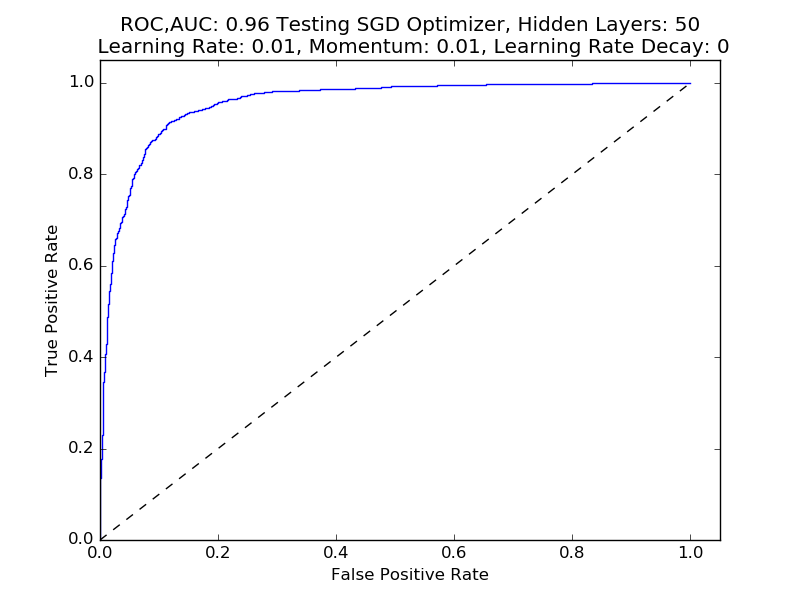
\includegraphics[width=1\textwidth]{/home/octopuscabbage/code/SpoofDetectionWithTransferCNN/roc_curves/SGD Optimizer, Hidden Layers: 50 Learning Rate: 0.01, Momentum: 0.01, Learning Rate Decay: 0/ROC,AUC: 0.96 Testing SGD Optimizer, Hidden Layers: 50 Learning Rate: 0.01, Momentum: 0.01, Learning Rate Decay: 0}
     }
     \hfill
     \subfloat[Validation\label{subfig-1:validation}]{%
       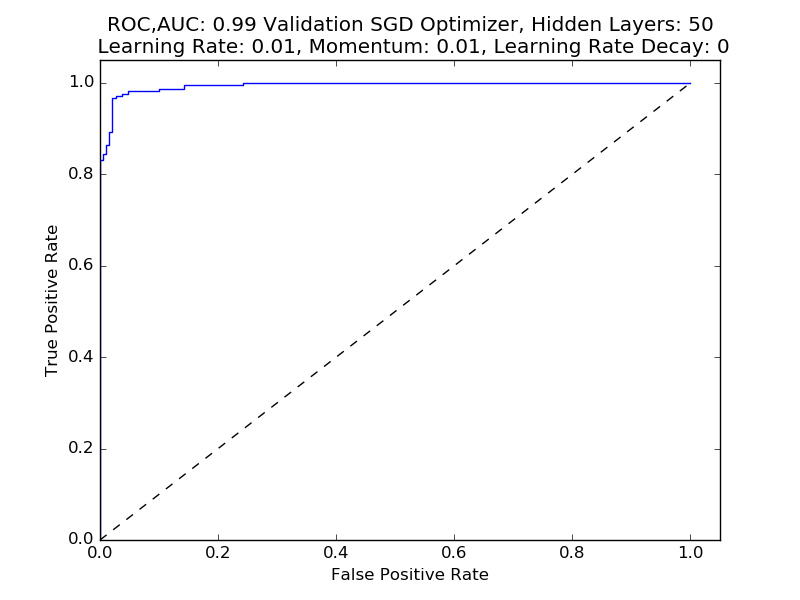
\includegraphics[width=1\textwidth]{/home/octopuscabbage/code/SpoofDetectionWithTransferCNN/roc_curves/SGD Optimizer, Hidden Layers: 50 Learning Rate: 0.01, Momentum: 0.01, Learning Rate Decay: 0/ROC,AUC: 0.99 Validation SGD Optimizer, Hidden Layers: 50 Learning Rate: 0.01, Momentum: 0.01, Learning Rate Decay: 0}
     }
     \caption{ROC Curves For Training On All Samples}
     \label{fig:dummy}
   \end{figure}

\begin{figure}
     \subfloat[Gelatine\label{subfig-2:gelatine}]{%
       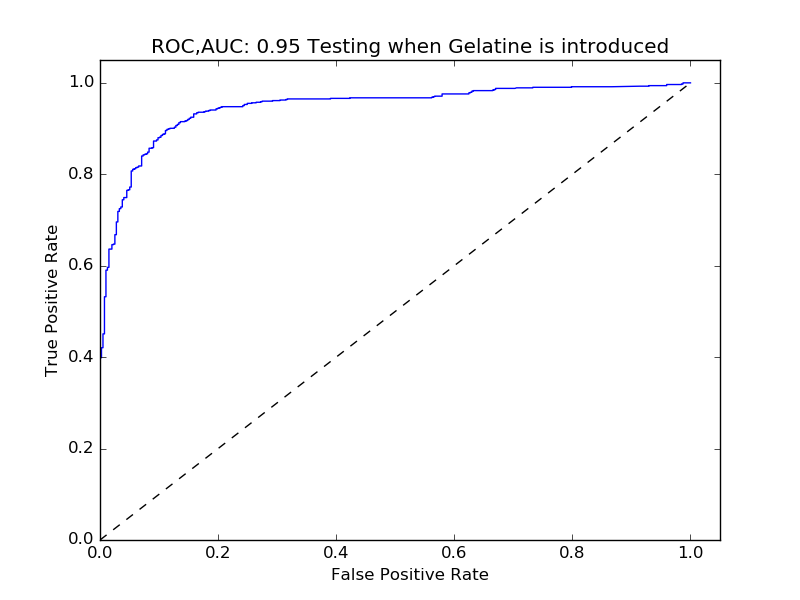
\includegraphics[width=0.6\textwidth]{/home/octopuscabbage/code/SpoofDetectionWithTransferCNN/roc_curves/Gelatine/ROC,AUC: 0.95 Testing when Gelatine is introduced}
     }
     \hfill
     \subfloat[Latex\label{subfig-2:latex}]{%
       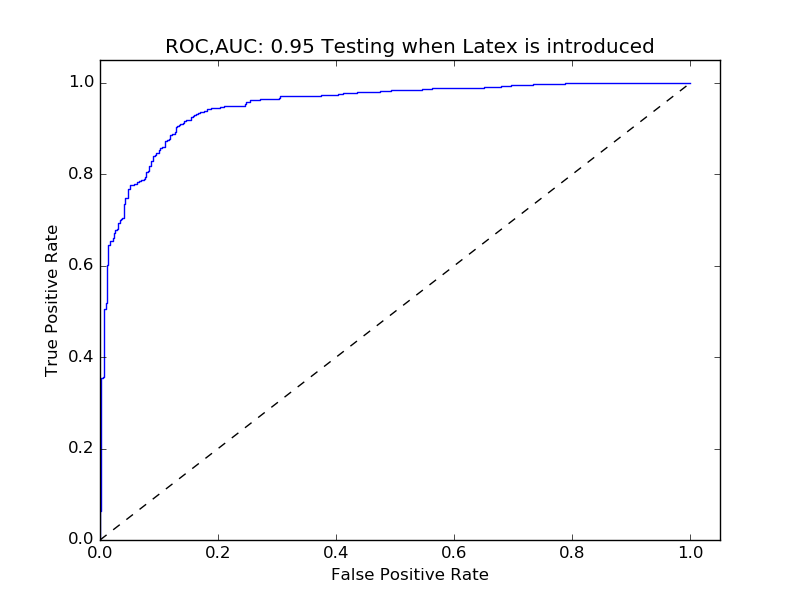
\includegraphics[width=0.6\textwidth]{/home/octopuscabbage/code/SpoofDetectionWithTransferCNN/roc_curves/Latex/ROC,AUC: 0.95 Testing when Latex is introduced}
     }
     \hfill
     \subfloat[Playdoh\label{subfig-2:playdoh}]{%
            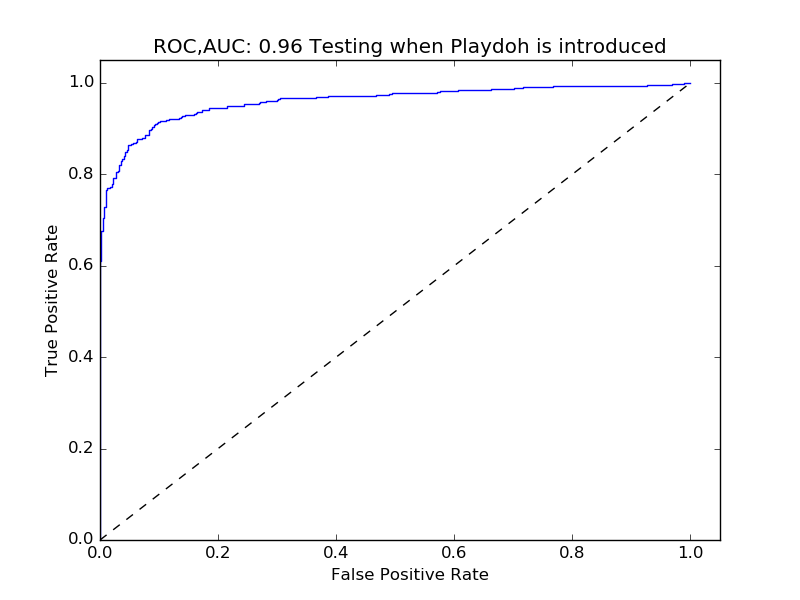
\includegraphics[width=0.6\textwidth]{/home/octopuscabbage/code/SpoofDetectionWithTransferCNN/roc_curves/Playdoh/ROC,AUC: 0.96 Testing when Playdoh is introduced}
    }
    \hfill
    \subfloat[Silicone\label{subfig-2:silicone}]{%
    	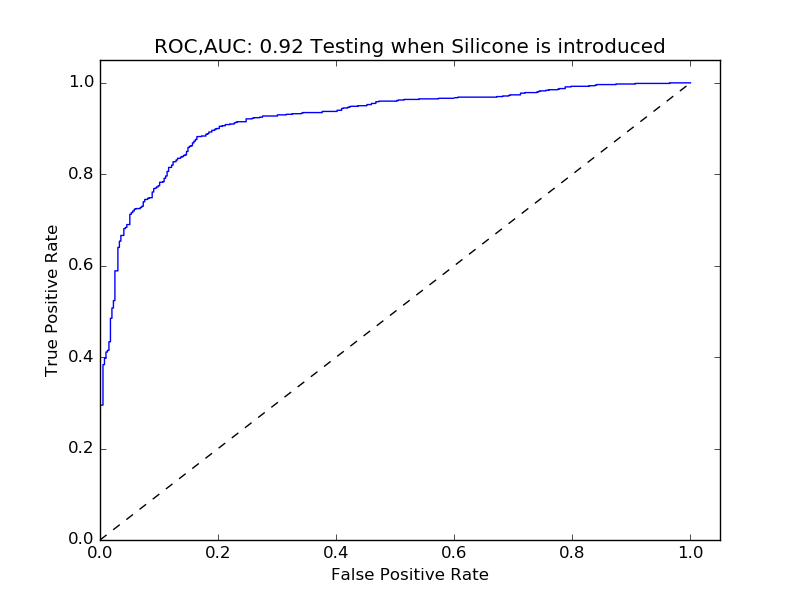
\includegraphics[width=0.6\textwidth]{/home/octopuscabbage/code/SpoofDetectionWithTransferCNN/roc_curves/Silicone/ROC,AUC: 0.92 Testing when Silicone is introduced}
    }
    \hfill
    \subfloat[Wood Glue\label{subfig-2:woodglue}]{%
         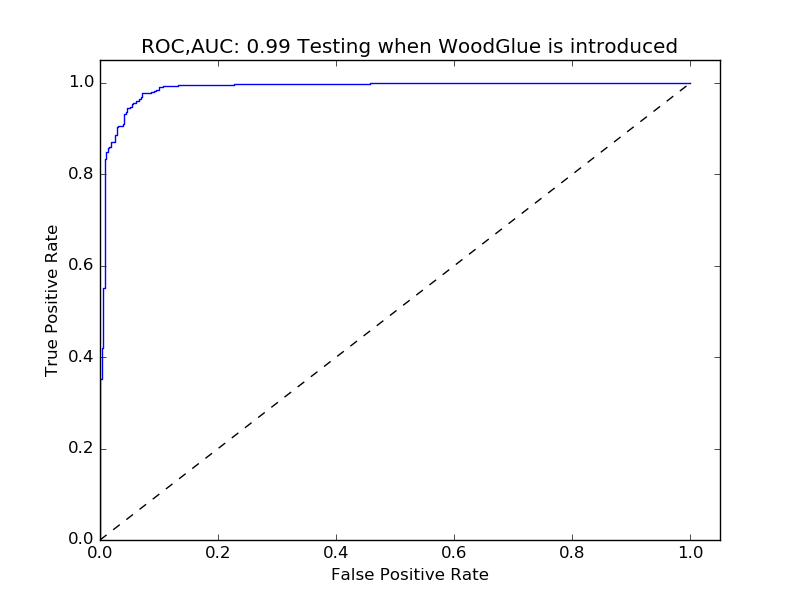
\includegraphics[width=0.6\textwidth]{/home/octopuscabbage/code/SpoofDetectionWithTransferCNN/roc_curves/WoodGlue/ROC,AUC: 0.99 Testing when WoodGlue is introduced}
     }
     \caption{ROC Curves When Novel Spoofs Are Introduced}
     \label{fig-2:dummy}
   \end{figure}
\pagebreak


\end{document}

